\documentclass{beamer}

\usepackage{hyperref}

%\usepackage{minted}

\usepackage{animate}

\usepackage{graphicx}

\def\Put(#1,#2)#3{\leavevmode\makebox(0,0){\put(#1,#2){#3}}}

\usepackage{color}

\usepackage{tikz}

\usepackage{amssymb}

\usepackage{enumerate}


\newcommand\blfootnote[1]{%

  \begingroup

  \renewcommand\thefootnote{}\footnote{#1}%

  \addtocounter{footnote}{-1}%

  \endgroup

}

\makeatletter

%%%%%%%%%%%%%%%%%%%%%%%%%%%%%% Textclass specific LaTeX commands.

 % this default might be overridden by plain title style

 \newcommand\makebeamertitle{\frame{\maketitle}}%

 % (ERT) argument for the TOC

 \AtBeginDocument{%

   \let\origtableofcontents=\tableofcontents

   \def\tableofcontents{\@ifnextchar[{\origtableofcontents}{\gobbletableofcontents}}

   \def\gobbletableofcontents#1{\origtableofcontents}

 }

%%%%%%%%%%%%%%%%%%%%%%%%%%%%%% User specified LaTeX commands.

\usetheme{Malmoe}

% or ...

\useoutertheme{infolines}

\addtobeamertemplate{headline}{}{\vskip2pt}



\setbeamercovered{transparent}

% or whatever (possibly just delete it)

\makeatother

\begin{document}
\title[Discussion 4 - Cryptography]{CS/MATH 111, Discrete Structures - Winter 2019. \\ Discussion 4 - Number Theory and Cryptography }
\author[CS111]{Andres, Sara, Elena}
\institute[Winter'19]{University of California, Riverside}
\makebeamertitle
\newif\iflattersubsect

\AtBeginSection[] {
    \begin{frame}<beamer>
    \frametitle{Outline} 
    \tableofcontents[currentsection]  
    \end{frame}
    \lattersubsectfalse
}

\AtBeginSubsection[] {
    \begin{frame}<beamer>
    \frametitle{Outline} 
    \tableofcontents[currentsubsection]  
    \end{frame}
}

\section{Euler's Totient}

\begin{frame}{Euler's Totient \footnote{For more info have a look at \url{https://tinyurl.com/kxtcf95}}}
The totient $\varphi(n)$ of a positive integer $n > 1$ is defined to be the number of positive integers less than $n$ that are coprime to $n$. 
    \begin{itemize}
        \item $\varphi(1)$ is defined to be 1.
        \item If the prime factorization of $n$ is given by: $n = p_1^{e_1}* \cdots *p_n^{e_n}$, then $\varphi(n) = n * (1 - \frac{1}{p_1}) * \cdots * (1 - \frac{1}{p_n})$.
        \item For example:
            \begin{itemize}
                \item $9 = 3^2$, so $\varphi(9) = 9 * (1 - \frac{1}{3}) = 6$
                \item $4 = 2^2$, so $\varphi(4) = 4 * (1 - \frac{1}{2}) = 2$
                \item $15 = 3 * 5$, so $\varphi(15) = 15 * (1 - \frac{1}{3}) * (1 - \frac{1}{5}) = 15*\frac{2}{3}*\frac{4}{5} = 8$
            \end{itemize}
      \end{itemize}
\end{frame}

\begin{frame}{Euler's Totient \footnote{For more info have a look at \url{https://tinyurl.com/y75o4ogh}}}
The totient $\varphi(n)$ of a positive integer $n > 1$ is defined to be the number of positive integers less than $n$ that are coprime to $n$. 
    \begin{itemize}
        \item When $n$ is a prime number, then $\varphi(n) = n - 1$.
        \item When $m$ and $n$ are coprime, then $\varphi(m*n) = \varphi(m) * \varphi(n)$.
        \item If $n$ is the product of two prime number, $p$ and $q$, then $\varphi(n) = (p - 1)*(q - 1)$.
        \item For example: $\varphi(15) = \varphi(3) * \varphi(5) = 2 * 4 = 8$.
      \end{itemize}
\end{frame}

\section{Problem 2}

\begin{frame}{Problem 2}
    \begin{itemize}
        \item ``Break'' RSA by guessing the factorization of $n$
        \item Compute Euler’s Totient Function $$\phi(n)$$ 
        \item Compute the decryption exponent $d$ by computing $$e^{-1} \pmod{\phi(n)}$$ solve this by enumerating.
        \item Using private key pair $(d,n)$, decrypt the messages by $$ M = C^{d} \pmod n$$ $C$ stands for the encrypted messages.
      \end{itemize}
\end{frame}

\begin{frame}{Problem 2}
    \begin{itemize}
        \item Show computation for 3 letters in \LaTeX: step-by-step, explaining everything;
        \item For the remaining message: \\
            Need to write a program (any language) -- Attach the program or compute by hand. All the computations attach (It is ok if written in pen).
        \item Decode the message
    \end{itemize}
\end{frame}

\section{Primes, congruent to $3 \pmod{4}$}

\begin{frame}{Infinitely many primes, congruent to $3 \pmod{4}$}
    \begin{itemize}
        \item Assume that $p_i = \{p_1, p_2, \cdots, p_k\}$, where $p_1 = 3$, are primes of the form: $$p_i \equiv 3 \pmod 4$$        \item We will construct a new one\footnote{ $N = 4 \cdot (p_1 \cdot p_2 \cdot \ldots \cdot p_k) + 3$ would also work.}           by looking at 
            $$N = 4 \cdot (p_1 \cdot p_2 \cdot \ldots \cdot p_k) - 1 $$
    \end{itemize}
\end{frame}

\begin{frame}{Infinitely many primes, congruent to $3 \pmod{4}$}
    \begin{itemize}
        \item $N = 4 \cdot (p_1 \cdot p_2 \cdot \ldots \cdot p_k) - 1 \equiv 3 \pmod{4}$
        \item Let $q$ be a prime factor of $N$, s.t. $q \mid N$, then:
        \begin{itemize}
            \item $q \not\equiv 0 \pmod 4$ \hspace{0.5cm} {\scriptsize [$q$ should not be prime]}
            \item $q \not\equiv 2 \pmod 4$ \hspace{0.5cm} {\scriptsize [$N$ is odd]}
            \item $q \not\equiv 3 \pmod 4$ \hspace{0.5cm} {\scriptsize [$q$ should be part of \{$p_1, p_2. \cdots, p_k$\}]}
            \item $q \equiv 1 \pmod 4$
        \end{itemize}
        \item Then, $N = q_1 \cdot q_2 \cdot \ldots \cdot q_t$ and $\forall i \in \{1,2,\cdots,t\}: q \equiv 1 \pmod{4}$.
        \item So, $N \equiv 1 \pmod{4}$, which is a contradiction of our initial definition of $N$.
    \end{itemize}
\end{frame}

\section{Conditions for parameters for RSA}

\begin{frame}{Conditions for parameters for RSA}
    What if ??? \\
    $gcd(e, \phi(n)) > 1$ 
    $$d \equiv e^{-1} \pmod{ \varphi(n)}$$
    $$e \cdot d \equiv 1 \pmod{\varphi(n)}$$
    \begin{itemize}
        \item p and q are small...
        \item $p = q$
        \begin{itemize}
            \item $\varphi(n) = (p-1)(q-1)$ ?
            \item $\varphi(n) = (p-1)(p-1)$ ???
        \end{itemize}
        \item Is double encription correct?
        \item Is double encription more secure?
    \end{itemize}
\end{frame}

\begin{frame}{Example}
    \centering
    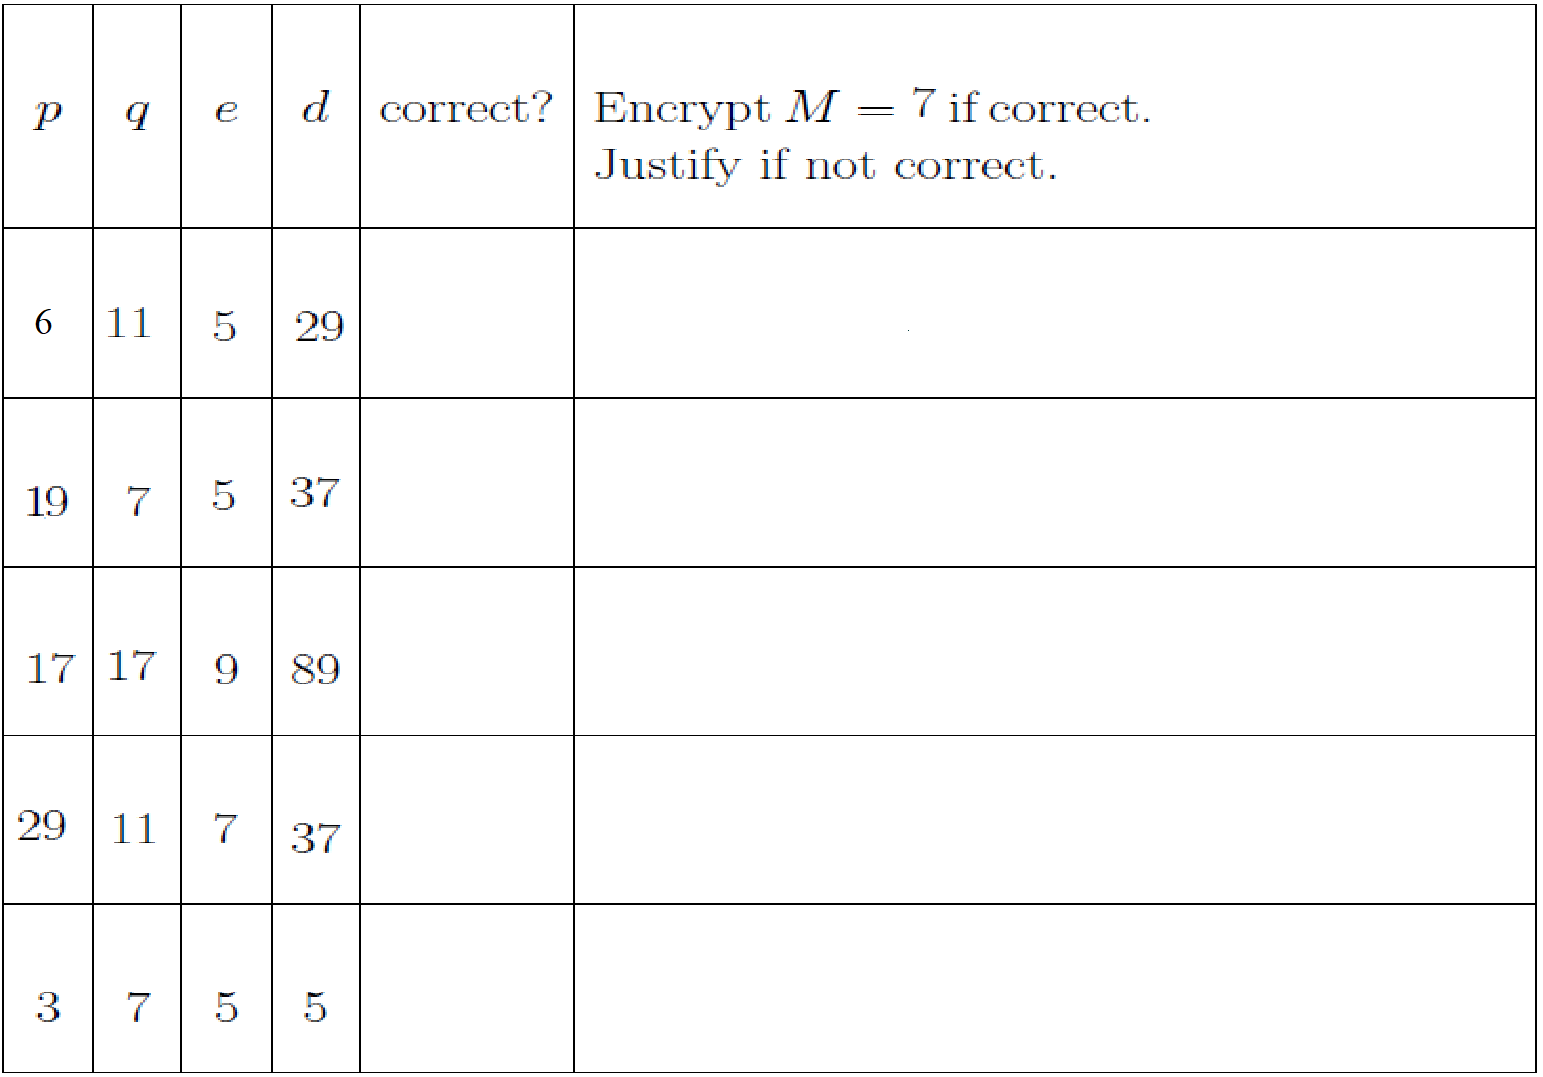
\includegraphics[width=.7\linewidth]{1.png}
\end{frame}

\begin{frame}{Example}
    \centering
    \begin{tabular}{|c|c|c|c|c|c|}
        \hline
         \textit{p}  & \textit{q}  & \textit{e}  & \textit{d}  & \textit{correct?} & \textit{Encrypt $M = 7$. Justify.}  \\ \hline
         6  & 11 & 5  & 29 & No       & 6 is not prime  \\ \hline
         19 & 7  & 5  & 37 & No       & $n = 133$ and $C = 7^5 \pmod{108} $  \\ \hline
         17 & 17 & 9  & 89 & No       & $p = q$  \\ \hline
         29 & 11 & 7  & 37 & No       & $e \cdot d \not\equiv 1 \pmod{\phi(n)} $  \\ \hline
         3  & 7  & 5  & 5  & Yes      & $n = 21$ and $C = 7^5 \pmod{12}$  \\ \hline
    \end{tabular}
\end{frame}

\section{Miller-Rabin Primality Test}

\begin{frame}{Miller-Rabin Primality Test}
    Primality is easy! \footnote{A nice intro to primality tests at \url{https://tinyurl.com/m2aksy7}}
    \begin{itemize}
        \item A primality test is a test or algorithm for determining whether an input number is prime.
        \item $N$ is prime if it has no divisors less or equal to $\sqrt{N}$.
        \item Most popular algorithms for primality testing are \textbf{probabilistic}; may output a composite number as a prime.
    \end{itemize}
\end{frame}

\begin{frame}{Miller-Rabin Primality Test\footnote{A great resource at \url{https://tinyurl.com/yafmmzax}}}
    \begin{itemize}
        \item Let $n$ be a prime number\footnote{$n > 2$}. Then $n - 1$ is even and we can write it as $2^{s} \cdot d$
        \item So we have: $$n - 1 = 2^{s} \cdot d$$where $s$ and $d$ are positive integers, and $d$ is odd. 
        \item For each $a$ in $(\frac{\mathbb{Z}}{n\mathbb{Z}})^{*}$, either...
        \begin{enumerate}
            \item $a^{d} \equiv 1 \pmod n$ or    
            \item $a^{2^r \cdot d} \equiv -1 \pmod n$, {\scriptsize For all $0 \leq r \leq s - 1$.}
        \end{enumerate}
        \item If we can find $a$, s.t. (1) and (2) are not true for all $r$, then $n$ is not prime.
    \end{itemize}
\end{frame}

\begin{frame}{Example}
Is $n = 221$ prime?
    \begin{itemize}
        \item We write $n - 1 = 220 = 2^2 \cdot 55$, so $s = 2$ and $d = 55$.
        \item We randomly select a number $a$ s.t. $1 < a < n - 1$. Let $a = 174$. 
        \item We proceed to compute:
        \begin{itemize}
            \item $a^{2^0 \cdot d} \mod n = 174^{55} \mod 221 = 47 \neq 1,- 1$
            \item $a^{2^1 \cdot d} \mod n = 174^{110} \mod 221 = 220 = -1$
        \end{itemize}
        \item Since $220 \equiv −1 \mod n$, either 221 is prime, or 174 is a \textbf{strong liar} for 221.
        \item Keep trying...
    \end{itemize}
\end{frame}

\begin{frame}{Example}
Is $n = 221$ prime?
    \begin{itemize}
        \item We write $n - 1 = 220 = 2^2 \cdot 55$, so $s = 2$ and $d = 55$.
        \item We try another random $a$, this time let $a = 137$:
        \begin{itemize}
            \item $a^{2^0 \cdot d} \mod n = 137^{55} \mod 221 = 188 \neq 1, -1$
            \item $a^{2^1 \cdot d} \mod n = 137^{110} \mod 221 = 205 \neq 1, -1$
        \end{itemize}
        \item Hence 137 is a \textbf{witness} for the compositeness of 221, and 174 was in fact a strong liar.
        \item Factors of 221 are 13 and 17.
    \end{itemize}
\end{frame}

\section*{Reference}

\begin{frame}{Reference}
    \begin{itemize}
        \item Discrete Mathematics and Its Applications. Rosen, K.H. 2012. McGraw-Hill. \\
        Chapter 4: Number Theory and Cryptography.
    \end{itemize}
\end{frame}

\end{document}
